% This is "sig-alternate.tex" V2.1 April 2013
% This file should be compiled with V2.5 of "sig-alternate.cls" May 2012
%
% This example file demonstrates the use of the 'sig-alternate.cls'
% V2.5 LaTeX2e document class file. It is for those submitting
% articles to ACM Conference Proceedings WHO DO NOT WISH TO
% STRICTLY ADHERE TO THE SIGS (PUBS-BOARD-ENDORSED) STYLE.
% The 'sig-alternate.cls' file will produce a similar-looking,
% albeit, 'tighter' paper resulting in, invariably, fewer pages.
%
% ----------------------------------------------------------------------------------------------------------------
% This .tex file (and associated .cls V2.5) produces:
%       1) The Permission Statement
%       2) The Conference (location) Info information
%       3) The Copyright Line with ACM data
%       4) NO page numbers
%
% as against the acm_proc_article-sp.cls file which
% DOES NOT produce 1) thru' 3) above.
%
% Using 'sig-alternate.cls' you have control, however, from within
% the source .tex file, over both the CopyrightYear
% (defaulted to 200X) and the ACM Copyright Data
% (defaulted to X-XXXXX-XX-X/XX/XX).
% e.g.
% \CopyrightYear{2007} will cause 2007 to appear in the copyright line.
% \crdata{0-12345-67-8/90/12} will cause 0-12345-67-8/90/12 to appear in the copyright line.
%
% ---------------------------------------------------------------------------------------------------------------
% This .tex source is an example which *does* use
% the .bib file (from which the .bbl file % is produced).
% REMEMBER HOWEVER: After having produced the .bbl file,
% and prior to final submission, you *NEED* to 'insert'
% your .bbl file into your source .tex file so as to provide
% ONE 'self-contained' source file.
%
% ================= IF YOU HAVE QUESTIONS =======================
% Questions regarding the SIGS styles, SIGS policies and
% procedures, Conferences etc. should be sent to
% Adrienne Griscti (griscti@acm.org)
%
% Technical questions _only_ to
% Gerald Murray (murray@hq.acm.org)
% ===============================================================
%
% For tracking purposes - this is V2.0 - May 2012

\documentclass{sig-alternate-05-2015}
\usepackage[brazil]{babel}
\usepackage[utf8]{inputenc}

\begin{document}

% Copyright
%\setcopyright{acmcopyright}
%\setcopyright{acmlicensed}
%\setcopyright{rightsretained}
%\setcopyright{usgov}
%\setcopyright{usgovmixed}
%\setcopyright{cagov}
%\setcopyright{cagovmixed}


% DOI
%\doi{10.475/123_4}

% ISBN
%\isbn{123-4567-24-567/08/06}

%Conference
%\conferenceinfo{PLDI '13}{June 16--19, 2013, Seattle, WA, USA}

%
% --- Author Metadata here ---
%\conferenceinfo{WOODSTOCK}{'97 El Paso, Texas USA}
%\CopyrightYear{2007} % Allows default copyright year (20XX) to be over-ridden - IF NEED BE.
%\crdata{0-12345-67-8/90/01}  % Allows default copyright data (0-89791-88-6/97/05) to be over-ridden - IF NEED BE.
% --- End of Author Metadata ---

\title{Sistema Vestível para Portadores de Deficiência Auditiva}
\subtitle{Sensory Expansion Vest for the Hearing Impaired}
%
% You need the command \numberofauthors to handle the 'placement
% and alignment' of the authors beneath the title.
%
% For aesthetic reasons, we recommend 'three authors at a time'
% i.e. three 'name/affiliation blocks' be placed beneath the title.
%
% NOTE: You are NOT restricted in how many 'rows' of
% "name/affiliations" may appear. We just ask that you restrict
% the number of 'columns' to three.
%
% Because of the available 'opening page real-estate'
% we ask you to refrain from putting more than six authors
% (two rows with three columns) beneath the article title.
% More than six makes the first-page appear very cluttered indeed.
%
% Use the \alignauthor commands to handle the names
% and affiliations for an 'aesthetic maximum' of six authors.
% Add names, affiliations, addresses for
% the seventh etc. author(s) as the argument for the
% \additionalauthors command.
% These 'additional authors' will be output/set for you
% without further effort on your part as the last section in
% the body of your article BEFORE References or any Appendices.

\numberofauthors{4} %  in this sample file, there are a *total*
% of EIGHT authors. SIX appear on the 'first-page' (for formatting
% reasons) and the remaining two appear in the \additionalauthors section.
%
\author{
% You can go ahead and credit any number of authors here,
% e.g. one 'row of three' or two rows (consisting of one row of three
% and a second row of one, two or three).
%
% The command \alignauthor (no curly braces needed) should
% precede each author name, affiliation/snail-mail address and
% e-mail address. Additionally, tag each line of
% affiliation/address with \affaddr, and tag the
% e-mail address with \email.
%
% 1st. author
\alignauthor Caique R. Marques
    \affaddr{Federal University of Santa Catarina}\\
    \affaddr{Florianópolis, Brazil}\\
    \email{c.r.marques@grad.ufsc.br}
% 2nd. author
\alignauthor Lucas R. Neis \\
    \affaddr{Federal University of Santa Catarina}\\
    \affaddr{Florianópolis, Brazil}\\
    \email{lucas.neis@grad.ufsc.br}
% 3rd. author
\alignauthor Rafael L. Cancian \\
    \affaddr{Federal University of Santa Catarina}\\
    \affaddr{Florianópolis, Brazil}\\
    \email{cancian@lisha.ufsc.br}
\and % use '\and' if you need 'another row' of author names
% 4th. author
\alignauthor Roberto A. P. Martins \\
    \affaddr{Federal University of Santa Catarina}\\
    \affaddr{Florianópolis, Brazil}\\
    \email{robertophi@gmail.com}    
}
% Just remember to make sure that the TOTAL number of authors
% is the number that will appear on the first page PLUS the
% number that will appear in the \additionalauthors section.

\maketitle
\begin{resumo}
    Este artigo foca na análise técnica de um Sistema Vestível para Portadores
    de Deficiência Auditiva. Usando motores de vibração presentes no colete,
    usamos comandos enviados de um smartphone para especificar um padrão de
    vibração para os motores (\texttt{e.g.} um sinal de bússola ou um áudio).
    Como é um sistema embarcado, ele é projetado para ser minimalista,
    portanto, ele tem que manter suporte às funcionalidades sem adição de
    hardware externo. Como este projeto usa uma FPGA, durante o
    desenvolvimento, nós focamos em fazer o software caber em uma memória
    \textit{in-chip}, como resultado, o software tem um tamanho de 30 KB.
\end{resumo}

\begin{abstract}
    This paper is focused in the technical analysis of a Sensory Expansion Vest
    for the Hearing Impaired. Using vibration motors attached to a vest, we use
    commands sent from a smartphone to specify a pattern of vibration to the
    motors (\texttt{e.g.} a compass signal or audio). As it is a embedded
    system, it is thought to be minimalist so it can support its features
    without the need of any extra hardware. As this project uses a FPGA, during
    development, we focused in making the software fit in the in-chip memory.
    As a result, the software has a size of 30KB.
\end{abstract}

%
% The code below should be generated by the tool at
% http://dl.acm.org/ccs.cfm
% Please copy and paste the code instead of the example below. 
%
% \begin{CCSXML}
% <ccs2012>
%  <concept>
%   <concept_id>10010520.10010553.10010562</concept_id>
%   <concept_desc>Computer systems organization~Embedded systems</concept_desc>
%   <concept_significance>500</concept_significance>
%  </concept>
%  <concept>
%   <concept_id>10010520.10010575.10010755</concept_id>
%   <concept_desc>Computer systems organization~Redundancy</concept_desc>
%   <concept_significance>300</concept_significance>
%  </concept>
%  <concept>
%   <concept_id>10010520.10010553.10010554</concept_id>
%   <concept_desc>Computer systems organization~Robotics</concept_desc>
%   <concept_significance>100</concept_significance>
%  </concept>
%  <concept>
%   <concept_id>10003033.10003083.10003095</concept_id>
%   <concept_desc>Networks~Network reliability</concept_desc>
%   <concept_significance>100</concept_significance>
%  </concept>
% </ccs2012>  
% \end{CCSXML}

% \ccsdesc[500]{Computer systems organization~Embedded systems}
% \ccsdesc[300]{Computer systems organization~Redundancy}
% \ccsdesc{Computer systems organization~Robotics}

%
%  Use this command to print the description
%
%\printccsdesc

% We no longer use \terms command
%\terms{Theory}

%\keywords{}

\section{Introdução}
    O desenvolvimento tecnológico possibilitou diversas melhorias ao estilo de
    vida, no entanto, ainda há problemas de adoção de inovações provindas de
    tal desenvolvimento por pessoas com deficiências porque a tecnologia não
    fora criada para atendê-las. Assim, ferramentas que fazem o uso de áudios
    acabam tendo difícil adoção por deficientes auditivos ou ferramentas com
    imagens e vídeos podem ser mais inacessíveis a deficientes visuais. Este
    projeto, baseado na proposta de David
    Eagleman\cite{eaglemanNewSensesHumans}, visa quebrar as barreiras de
    comunicação usando o que qualquer pessoa é capaz de notar: o tato. Graças
    ao tato, podemos transformar sinais que são impossíveis de serem notados
    por alguém com alguma deficiência sensorial em um sinal facilmente
    entendível usando vibrações. Através de um colete de motores, um sinal é
    enviado a partir de um smartphone e o usuário é capaz de sentir o comando
    que ele enviou através de um padrão de vibração estabelecido (um certo tipo
    de vibração para recepção do áudio ou um certo tipo de vibração para a
    localização da coordenada norte).

    Atualmente, o projeto já tem suporte a áudio, giroscópio e bússola. Nesta
    versão do software empregado, infelizmente, a adição de novos atributos é
    trabalhosa, mas uma nova versão do software está sendo trabalhada para que
    isso não seja uma tarefa árdua. Graças ao uso de uma FPGA, o hardware, por
    ora, é maleável o bastante para podermos mexer com as configurações e
    obtermos um melhor resultado. Em seu estado atual, o hardware conta com um
    controlador para a matriz de motores, um processador Nios II, uma UART e um
    timer.
    
    Nas próximas seções iremos detalhar quais os componentes de hardware usados
    para a realização deste projeto e como a comunicação é feita entre software
    e hardware. Em seguida, cada componente de software é explicado. Por fim,
    apresentaremos as ideias futuras do projeto, que envolve a reimplementação
    do software, que já está em seus estados iniciais.

\section{Hardware e Periféricos}
    O hardware é, em essência, uma FPGA (\textit{Altera DE2}) com diversos
    componentes.\footnote{Esta seção é um esboço. A adesão de explicações por
    parte dos responsáveis pelo hardware é necessária.}

\section{Software}
\label{sec:SW}

    O software é, neste momento, simples e busca apenas o controle dos
    mecanismos da camada de hardware. No entanto, o código lida com instruções
    diferentes e, portanto, podemos separar seus blocos de funcionamento.
    
    Apesar de ingênuo, o software em seu estado atual tem dois níveis para
    controlar os componentes de hardware. A primeira camada, mais próxima ao
    hardware — doravante chamada de camada de mediação — e a segunda camada,
    acima da camada de mediação — doravante chamada de camada de controle e
    aplicação.

    A camada de mediação é responsável pelas interações com o hardware e,
    portanto, quaisquer usos de componentes passam por esta seção. Junto aos
    drivers provindos pela Altera\cite{downloadCenter} para controle de
    componentes, a camada de mediação, se torna a nossa \textit{Hardware
    Abstraction Layer} (\textit{HAL}) ou Camada de Abstração de Hardware.

    Já a camada de controle e aplicação é responsável pela interpretação de
    sinais provindos de comandos do smartphone e geração de padrões para
    vibração. Atualmente, há apenas três padrões de vibração estabelecidos:
    Áudio, Bússola e Giroscópio.
    
    \subsection{A Camada de Mediação}
        Na camada de mediação, se faz o controle dos seguintes componentes de
        Hardware: \textit{Fast Fourier Transform} (FFT), \textit{Motores} e
        \textit{Wi-Fi}. Cada um desses componentes só pode ser acessado através
        dessa camada e pelos seus devidos controladores (ou mediadores). Nesta
        seção explicamos cada um dos mediadores.
        \subsubsection{FFT}
        \label{sec:FFT}
            Infelizmente o componente para a execução da Transformada de
            Fourier ainda não foi implementado. Como consequência, o mediador
            da FFT atua apenas como um mediador para um componente Dummy.
            
            Sendo assim, recebendo um arranjo de $n$ amostras, este mediador
            apenas retorna metade dos mesmos sem qualquer escolha ou
            processamento.

        \subsubsection{Motores}
            A matriz de motores no colete recebe e realiza comandos provindos
            de uma classe específica, que é o mediador dos motores. Os
            comandos, são de tamanho de 32 bits, têm quatro campos que são:
            comando (bits 31 a 24), linha (bits 23 a 16), coluna (bits 15 a 8)
            e valor (bits 7 a 0). A seguir, mais detalhes de cada campo:
            \begin{itemize}
                \item \textbf{Comando}: Especifica como deve ser a vibração
                    pelos motores, se a vibração deve ser gradual até a um
                    ponto específico ou se a vibração deve diminuir
                    gradualmente até parar. Segue-se os cinco comandos criados:
                \begin{itemize}
                    \item Especificar potência (\texttt{0x0}): este comando
                        especifica ou muda a potência de vibração de um dado
                        motor alvo, especificado pelos campos "linha" e
                        "coluna" do comando;
                    \item Especificar taxa de aumento de potência
                        (\texttt{0x1}): a potência vai aumentando gradualmente
                        até atingir o limite especificado no campo
                        \texttt{Valor} (veja mais adiante);
                    \item Especificar taxa de decaimento (\texttt{0x2}): a
                        potência vai decaindo gradualmente até atingir o limite
                        especificado no campo \texttt{Valor} (veja mais
                        adiante);
                    \item Cópia de uma linha a outra (\texttt{0x3}): este
                        comando copia todos os valores dos motores de uma linha
                        para a de baixo;
                    \item Cópia de uma coluna a outra (\texttt{0x4}): este
                        comando copia todos os valores dos motores de uma
                        coluna para a coluna à direita;
                \end{itemize}
                
                \item \textbf{Linha}: Especifica qual a linha, da matriz de
                    motores, deve ser escrita. Se o valor for 255, toda a linha
                    é selecionada para escrita;
                
                \item \textbf{Coluna}: Especifica qual a coluna, da matriz de
                    motores, deve ser escrita. Se o valor for 255, toda a linha
                    é selecionada para escrita;
                
                \item \textbf{Valor}: Define qual a intensidade máxima de
                    vibração dos motores, caso o valor do comando seja
                    \texttt{0x02}, o limite especificado neste campo é o máximo
                    que a vibração deve alcançar.
                
            \end{itemize}
            Ressalta-se aqui que o controle desses comandos é todo feito em
            hardware.

        \subsubsection{Wi-Fi}
            A comunicação entre o smartphone e o colete de motores é via rede
            Wi-Fi. Conforme especificado na seção anterior, o hardware suporta
            recebimento de pacotes via Wi-Fi que é interpretado pelos
            mediadores e respondido pela matriz de motores, assim, cada pacote
            recebido contém um caractere correspondente que identifica qual
            mediador deve ser ativado e quais os parâmetros que ele deve
            obedecer.
            
    \subsection{A Camada de Controle e Aplicação}
        Como mencionado na seção~\ref{sec:SW}, esta camada lida com os padrões
        de vibração e a análise de dados recebidas pelo smartphone. Todos os
        dados são enviados via Wi-Fi, sendo essa camada a responsável por
        iniciar a espera por um novo sinal de dados, a escolha de qual é o
        processamento necessário e padrão de vibração a ser executado. Cada
        tipo de dados é identificado por uma letra enviada junto ao sinal de
        dados. Nesta seção explicamos como funcionam cada um dos padrões e os
        processamentos usados.

        \subsubsection{Áudio}
            Quando recebido do mediador do Wi-Fi, a string de dados de tamanho
            $n$ recebida contém $n-1$ amostras de áudio enviadas pelo
            smartphone e o seu primeiro caractere é \texttt{a} que identifica
            os dados como áudio. A primeira medida é enviar os dados para o
            mediador da FFT (aprofundado na subseção~\ref{sec:FFT}). O retorno
            do mediador é um arranjo de $\frac{n-1}{2}$ inteiros —
            supostamente, frequências em um intervalo de [$0$, $n-1$] — que
            deve ser enviado para o gerador de vibração de áudio (GVA).
            
            O padrão de vibração do áudio é simples. Uma vez que o primeiro
            arranjo de frequências é enviado para o GVA, este divide o número
            $n-1$ de frequências pelo número $l$ de motores em uma linha. Este
            valor é o número de frequências que cada motor é responsável.
            
            \begin{gather*}
                s = \frac{n-1}{l}
            \end{gather*}
            
            Portanto, cada motor da linha administra $s$ frequências. Assim, o
            primeiro motor da linha (motor da coluna $0$) lida com as
            frequências em [0, $s$), já o segundo lida com as frequências em
            [$s$, $2\times s$) e assim em diante.
            
            Para definir a potência em que o motor deve vibrar, é feito então a
            média aritmética dos valores das $s$ frequências em que o motor $i$
            é responsável.
            
            Quando um arranjo chega ele é, inicialmente, aplicado na primeira
            linha de motores de cima para baixo (\texttt{i.e.} a linha $0$). Os
            dados que estavam sendo tocados anteriormente são empurrados para a
            linha de baixo. Com isso, gera uma linha de áudios que foram
            tocados ao longo do tempo.
            
            A taxa de aumento de potência é de 5 e a taxa de decaimento é de 1.

        \subsubsection{Bússola}
            Como sabemos, uma bússola nos mostra onde está o norte, portanto, o
            que é recebido via Wi-Fi do smartphone é a direção, em graus, em
            que o norte está. Além disso, também é enviado o caractere
            identificador \texttt{c} (de \textit{compass}).
            
            Diferente do áudio, nenhum pré-processamento é necessário. No
            entanto, cálculos ainda são necessários para escolher quais motores
            devem ser ativados. Existem duas diferentes versões para o padrão
            de vibração da bússola: uma usando cinco motores (quatro em uma
            mesma linha e mais um na linha acima desta) e um segundo que usa
            nove motores (oito em uma mesma linha e mais um na linha acima
            desta) chamadas de \texttt{compass4} e \texttt{compass8},
            respectivamente. Ambas são explicadas a seguir:
            
            \begin{itemize}
                \item \textbf{compass4:} Esta versão é usada quando há no
                    mínimo quatro e no máximo sete motores em uma linha de
                    motores. No entanto, são necessários cinco motores. Um
                    motor para indicar que o ângulo está entre 355$^\circ$ e
                    5$^\circ$ e quatro outros para indicar os quadrantes em que
                    o ângulo pode está. O motor que indica que o usuário já
                    olha para o norte (cujo chamamos de motor \texttt{N}) se
                    localiza na linha de motores acima da última linha(número
                    de motores por coluna $- 1$) que é onde os demais motores
                    estão.
                
                A imagem a seguir ilustra a ideia:
                \begin{figure}[h!]
                    \centering
                    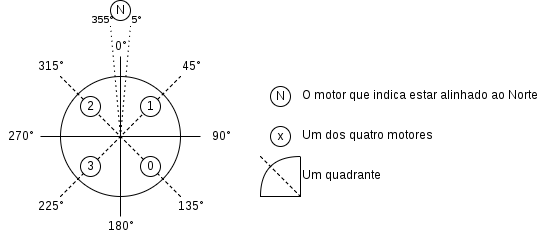
\includegraphics[scale=0.45]{imgs/compass4.png}
                    \caption{Representação dos quadrantes que os motores
                    assumem na arquitetura \texttt{compass4}}
                    \label{fig1}
                \end{figure}
                
                
                Então, conforme a figura \ref{fig1}, se o ângulo recebido
                    estiver no intervalo (0$^\circ$, 90$^\circ$] o motor na
                    coluna 1 deve ser ativado. Caso o ângulo estiver em
                    [270$^\circ$, 0$^\circ$), o motor na coluna 2 deveria ser
                    ativado.
                
                No entanto, se o motor estiver em [355$^\circ$, 0$^\circ$) o
                    motor \texttt{N} será ativado juntamente ao motor na coluna
                    2. Similarmente, se o motor estiver em (0$^\circ$,
                    5$^\circ$] o motor \texttt{N} será ativado juntamente ao
                    motor na coluna 1. O motor \texttt{N} só será ativado
                    sozinho caso o ângulo seja exatamente 0$^\circ$. Com isso,
                    um usuário consegue saber se precisa virar mais para a
                    esquerda ou mais para a direita para localizar o norte.

                \item \textbf{compass8:} Esta implementação é uma adaptação da
                    versão \texttt{compass4} e deve ser usada caso hajam pelo
                    menos 8 motores por linha. A diferença dessa versão é o
                    melhor uso do maior número de motores para identificar um
                    maior número de intervalo de ângulos. A imagem a seguir
                    ilustra a ideia:
                \begin{figure}[h!]
                    \centering
                    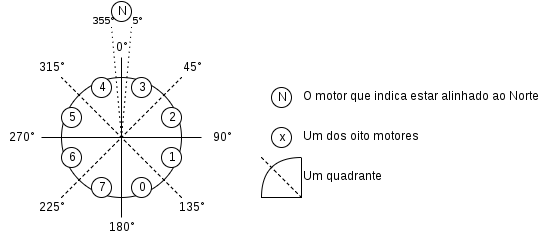
\includegraphics[scale=0.45]{imgs/compass8.png}
                    \caption{Representação dos setores que os motores assumem na arquitetura \texttt{compass8}}
                    \label{fig2}
                \end{figure}
                
            \end{itemize}
            
            O método usado é selecionado em tempo de compilação, através do uso
            de um \texttt{if-then-else} metaprogramado.
            
            A taxa de aumento de potência é de 5 e a taxa de decaimento é de 1.
            Além disso, a potência do motor é fixa, originalmente, em 25.
            
        \subsubsection{Giroscópio}
            Giroscópios nos fornecem a aceleração angular em três eixos. Para
            tornar isso em um padrão de vibração em uma matriz de duas
            dimensões, usamos a aceleração em dois desses eixos para selecionar
            um motor e a terceira se torna a potência em que o motor deve
            vibrar.
            
            Mas para fazermos isso, temos alguns problemas. Se o número de
            motores em uma das dimensões for par, ele deverá ser tratado
            diferente do que seria se o número de motores fosse ímpar. Além
            disso, precisamos definir um intervalo de atuação.
            
            Para resolver isso, separamos em dois métodos. O primeiro é usado
            para quando temos um conjunto de motores ímpar em certa dimensão.
            Este funciona por encontrar o motor localizado no centro desta
            dimensão. Com isso, definimos nosso intervalo de atuação para
            valores entre -100 e 100. Separamos, então, dois motores para
            representar valores fora dos limites e o restante dos motores
            dividem os 200 de intervalo entre si.
            
            \begin{gather*}
                intvpmtr = \frac{200}{m-2}
            \end{gather*}
            
            Onde m é o número de motores na dimensão onde trabalhamos.
            Com isso, o intervalo por motor é definido e podemos então saber
            que o motor 0 da dimensão em questão lida com o intervalo $(-100,
            intvpmtr-100]$ e assim por diante. Mais importante, podemos definir
            que o motor localizado no centro da dimensão lida com
            $[-\frac{intvpmtr}{2}, \frac{intvpmtr}{2}]$.
            
            Logo, iniciamos testando se o valor está dentro do intervalo do
            motor central. Se sim, sabemos que o motor está na parte central da
            dimensão procurada. Caso contrário, testamos se o valor é negativo.
            Se sim, procuramos o motor que deve lidar com este valor entre os
            motores negativos, do contrário testamos entre os motores que lidam
            com os valores positivos.
            
            No entanto, a versão com um número par de motores na dimensão não
            tem um motor no centro, então é feita uma busca simples para
            encontrar o motor que lida com o intervalo em que o valor está
            compreendido.
            
            Sendo assim, basta tratar a dimensão remanescente. Esta é tratada
            de maneira simples. Pegamos o valor absoluto e então testamos para
            verificar se esta é menor que 240 (pois 255 é a maior potência que
            um motor sabe lidar), caso positivo, apenas somamos 10 a esse valor
            e temos, portanto, todos os valores necessários. Por outro lado, se
            for maior que 240, apenas reduzimos para 240 e somamos 10.
            
            A taxa de aumento de potência é de 15 e a taxa de decaimento é de 5.
        
        \subsubsection{Escalonamento de Padrões}
            Um problema persistente neste projeto é o caso em que dois sinais
            são enviados a um mesmo motor. Uma das formas de contornar o
            problema é reservando fatias de tempo para cada sinal usar o motor,
            método chamado de multiplexação temporal. A forma implementada no
            projeto consiste num timestamp que é iniciado, e após meio segundo,
            o sinal é alternado para usar o motor.

        \subsubsection{Adição de Novos Padrões}
            A atual implementação torna difícil a adição de novos padrões. No
            entanto, a remodelagem do software pensa em tornar o processo fácil
            e sem complicações. No estado corrente, é necessário entender
            verdadeiramente o que acontece na camada de controle e aplicação.

\section{Remodelagem do Software}
    Uma proposta de remodelagem do software foi feita e os primeiros passos
    foram dados. A ideia é a reformulação do projeto em camadas, onde cada uma
    tem suas funções. O projeto será dividido em três camadas: hardware,
    sistema operacional e aplicação.
    
    \begin{figure}[h!]
        \centering
        \includegraphics[scale=0.28]{imgs/new_class_diagram.png}
        \caption{Diagrama de classes do projeto reformulado}
        \label{fig:classDiagram}
    \end{figure}
    
    \begin{itemize}
        \item \textbf{Hardware}: Parte mais baixo nível, correspondendo toda a
            parte de hardware do projeto, logo, componentes desta camada são a
            UART, o Wi-Fi e a matriz de motores;
        \item \textbf{Sistema operacional}: Será a camada responsável em fazer
            a comunicação entre a camada de aplicação com o hardware, portanto,
            componentes nesta camada são os mediadores;
        \item \textbf{Aplicação}: Camada responsável com a recepção dos dados
            especificados pelo usuário, tal qual padrão usar, e da
            administração dos padrões, como o pacote recebido deve ser tratado
            pela aplicação e respostas vindas da conexão Wi-Fi estabelecida.
    \end{itemize}
    
    O diagrama de classes na figura \ref{fig:classDiagram} descreve a estrutura
    da remodelagem do projeto.

    A meta é que cada componente realize apenas uma, e muito bem, dada tarefa.
    Além disso, a proposta é deixar o projeto extensível, que o torne mais
    fácil de adicionar novos recursos, como por exemplo, ao adicionar um novo
    componente de coleta de dados - simplesmente fazer com que a classe nova
    seja filha de \texttt{DataHandler}, assim, esta classe, através do padrão
    de cadeia de responsabilidade, pergunta a qual das classes filhas é apta
    para executar a tarefa que recebeu do aplicativo de smartphone (ou seja,
    pelo usuário).

\nocite{niosHandbook}
\bibliographystyle{abbrv}
\bibliography{reference}

\end{document}
